\chapter{绪论}
\label{Intro}

\section{研究背景}

\subsection{社交媒体}
作为划时代的创新,互联网20年以来已深刻影响和改变着我们的生活,思维和行为方式。尤其现在,我们可以通过手机、各种穿戴式智能设备,随时随地保持与互联网不间断联系。根据中国互联网络信息中心的权威报告,截至2014年7月,我国网民规模达6.41亿,手机网民规模已超过5亿,互联网普及率为47.4\%\footnote{\url{http://www.cnnic.cn/hlwfzyj/hlwfzzx/qwfb/201408/t20140825\_47878.htm}}。
随着互联网技术的迅猛发展,出现了形形色色吸引用户参与的社交媒体(Social Media)平台,并且已经成为人类工作、学习、生活必不可少的重要部分。图~\ref{fig1-1}展示了各种国内外的在线社交媒体平台。

\begin{figure}[htp]
\centering
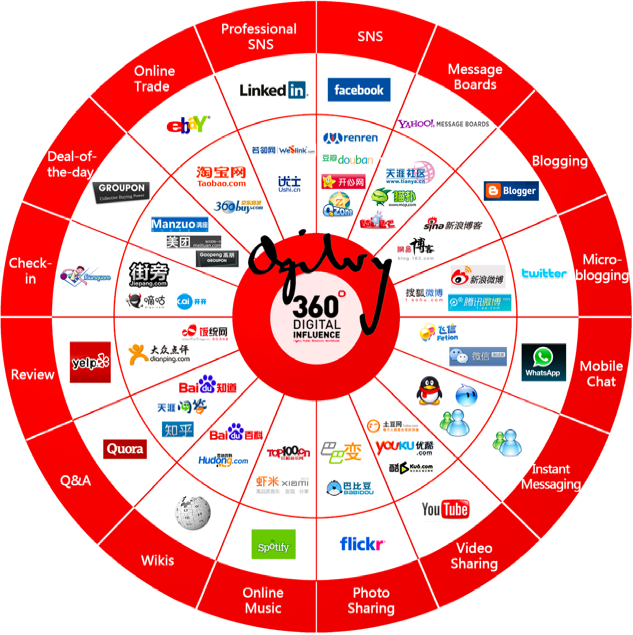
\includegraphics[height=220pt]{1-1.png}
\caption{国内外社交媒体}
\label{fig1-1}
\end{figure}

社交媒体中的互联网用户不再是单纯的信息接收者,同时也是网络内容的制造者,人们通过社交媒体进行交流而获取和产生信息。以中国为例,目前拥有12亿手机用户、5亿微博用户、5亿微信用户,每天信息发送量超过200亿条,交流无处不在、无时不有。表~\ref{tab1-1}是互联网网站流量信息公司Alexa\footnote{网站地址:\url{www.alexa.com},访问时间:2014年9月。}统计的网络访问统计,从表中可以看出,根据统计,流量前十的互联网网站中社交媒体占了绝大部分。

\begin{table}[htp]
\centering
\caption{Alexa统计访问量前十名网站}
\label{tab1-1}
\begin{threeparttable}
 \begin{tabular}{|l|l|l|l|}
 \hline
 排名&网站&排名&网站\\
 \hline
 1& Google.com& 6&\textbf{ Wikipedia.org\tnote{1}}\\
 2& \textbf{Facebook.com}& 7& \textbf{Amazon.com}\\
 3& \textbf{Youtube.com}& 8& \textbf{Twitter.com}\\
 4& Yahoo.com& 9& \textbf{Qq.com}\\
 5& Baidu.com& 10& \textbf{Taobao.com}\\
 \hline
\end{tabular}
\begin{tablenotes}
  \centering
  \footnotesize
\item[1]表中加黑部分为社交媒体
\end{tablenotes}
\end{threeparttable}
\end{table}

那么究竟什么是社交媒体呢?社交媒体的典型代表维基百科是这样定义的\footnote{\url{http://en.wikipedia.org/wiki/Social media/}}:

\begin{definition}[Social Media]
Social media are media for social interaction, using highly accessible and scalable communication techniques. It is the use of web-based and mobile technologies to turn communication into interactive dialogue.
\end{definition}
从定义中我们可以看出,社交媒体是以互联网的思想和技术为基础的一项应用,用户可以借此进行内容创作、情感交流与信息分享。一般来讲,社交媒体可以分为如表~\ref{tab1-2}所示的几种类型:

\begin{table}[htp]
\centering
\caption{社交媒体的类型}
\label{tab1-2}
 \begin{tabular}{|l|l|}
 \hline
 类型& 代表性网站\\
 \hline
 维基(Wiki) & Wikipedia,Scholarpedia,百度百科\\
 \hline
 博客(Blogging) & Blogger,LiveJournal,WordPress,博客\\
 \hline
 新闻(Social News) & Digg, Mixx,Slashdot\\
 \hline
 微博(Micro Blogging) & Twitter,Google Buzz,新浪微博\\
 \hline
 评论(Opinion \& Reviews) & ePinions,Yelp,豆瓣\\
 \hline
 问答(Question Answering) & Yahoo! Answers,百度知道\\
 \hline
 媒体分享(Media Sharing) & Flickr,Youtube,优酷\\
 \hline
 书签(Social Bookmarking) & Delicious,CiteULike\\
 \hline
 社交网络(Social Networking) & Facebook,LinkedIn,MySpace,人人网\\
 \hline
\end{tabular}
\end{table}

从表中可以看出,社交媒体有多中不同类型,因此会产生多种不同形式的信息,包括文本、图像以及视频等。社交媒体上的信息由广大的社交媒体使用者产生,因此称为用户产生内容(User-Generated Content,UGC),这些信息依靠用户之间的关系与交互形成相互关联的庞大数据库。Kaplan和Haenlein\upcite{Kaplan2010}从数据和信息流动角度讨论了社交媒体:首先是作为媒体(media),社交媒体中最突出的特点是它区别于电视、广播和报纸等传统媒体(信息的流动是从少数内容生产者到广大的信息消费者),内容产生的权利扩展到了所有的用户,而且信息流动的方式变得不确定,用户可以在内容消费者和生产者之间多次瞬间改变自己的角色;其次,作为社交工具,我们称这种新媒体是社会化的(social)的媒体,社会化意味着信息内容不只是由个体用户产生,更多是与其他用户的协作产生,因此信息的内容变得更加多样化,因此社交媒体不只是用来产生信息,也为用户间互相交流通信以及传播信息的便利工具。

虽然社交媒体的出现为我们信息交流提供了便利,但是随着用户数量不断增加,产生的内容达到新的量级,导致我们作为信息消费者遇到了一些新的挑战,使得我们从“信息海洋”中找到有用信息变得更加困难,这通常称为信息超载(information overload)\footnote{信息超载描述了一种状态,就是当一个人在做选择时因为太多的信息而造成决策的困难。}。同时,由于社交媒体发布消息相对廉价和方便,内容产生门槛降低,任何人都能够参与其中,因此社交媒体中的数据出现了不同于传统媒体数据的新特点。
一般来讲,社交媒体中的数据具有以下特点\upcite{eisenstein2013bad}:
\begin{itemize}
\item \textbf{数量巨大(Big):}社交媒体中每个用户产生的数据可能不大,但是作为用户群体数量庞大,整体数据规模不可小觑,比如平均每天有超过300万条的微博(tweets)发布到Twitter\footnote{\url{http://www.twitter.com/}},每分钟有超过3000张照片上传到Flickr\footnote{\url{http://www.flickr.com/}},每年有超过160多万的博客(blogs)发表。
\item \textbf{广泛链接(Linked):}社交媒体的社会化特性使得用户产生的数据天生就是广泛链接的,最直观的就是用户产生内容往往由于用户之间的各种社交关系链接在一起,是一种新形式的大数据。这种链接的数据显然不是独立同分布的(IID,independent and identically distributed),对于想要使用传统的数据挖掘和机器学习方法研究社交媒体的研究人员是一种挑战\upcite{jensen2002linkage,taskar2003label}。
\item \textbf{充满噪声(Noisy):}社交媒体数据产生门槛的降低以及接入手段的增加,使得社交媒体的数据质量参差不齐,充满噪声\upcite{Agichtein2008}。不仅于此,社交媒体中的网络结构也充满噪声,一是网络中存在一些传播虚假和垃圾信息的用户\upcite{stringhini2010detecting},二是用户间建立关系的便捷性使得用户很容易将各种社会关系混杂在一起,无法区分好朋友和陌生人\upcite{xiang2010modeling}。
\item \textbf{非结构化(Unstructured):}社交媒体中用户产生数据,主要是文本数据是高度非结构化的,尤其是随着移动互联方式的普及,越来越多的用户使用移动设备更新Facebook的状态,发送微博,或者回复别人的帖子,这不但导致了文本内容短小,而且错误拼写频繁出现\upcite{rossion1999spatio},经常还有一些非自然语言的使用,比如表情符(:),:()和缩写(h r u?)等\upcite{speriosu2011twitter}。
\item \textbf{不完整性(Incomplete):}为了保护用户的隐私,社交媒体平台一般允许用户将其一些个人数据进行隐藏不被他人看到,这些数据包括个人信息,状态更新,朋友列表,发布的视频和照片以及与他人的信息交流等。比如Facebook仅有很少部分用户(小于1\%)公开了他们的个人数据\upcite{mislove2010you}。因此社交媒体的数据是极度不完整和稀疏的。
\end{itemize}

社交媒体的迅速普及与壮大,使得它在政治、经济、教育、社会等多方面发挥着越来越重要的作用。一些拥有互联网公司开始以社交媒体大数据资源为支撑,以SaaS形式为用户提供服务。典型的如谷歌和Facebook的的自助式广告下单服务系统、Twitter基于实时搜索数据的产品满意度分析以及国内百度推出的大数据营销服务 “司南”等。同时,政府也是社交媒体数据的积极使用者,2013年曝光的棱镜门事件显示出美国国家安全部门在使用社交媒体数据应用的强大实力,其应用范围之广、水平之高、规模之大都远远超过人们的想象。白宫2014年5月发布的《大数据:抓住机遇,守护价值》报告中重点提及了社交媒体大数据\footnote{来源:\url{http://www.whitehouse.gov/sites/default/files/docs/big\_data\_privacy\_report\_may\_1\_2014.pdf}}。
社交媒体大行其道的今天,自然也会成为品牌营销的手段之一,比如今年世界杯的主要赞助商之一可口可乐就首次挑选了粉丝在Facebook\footnote{\url{http://www.facebook.com/}}和Twitter上分享的照片,尝试进行iBeacon在社交媒体营销中的运用。
目前常见的社交媒体的大数据应用有:
一是基于用户个人信息、行为、位置、微博等数据而进行的个性化推荐、交叉推荐、品牌监测等营销类大数据应用,被互联网广告、电子商务、微博、视频、相亲等公司普遍采用。
第二,公共服务类大数据应用,即不以盈利为目的、侧重于为社会公众提供服务的大数据应用。典型案例如谷歌开发的流感、登革热等流行病预测应用能够比官方机构提前一周发现疫情爆发状况。国内也有搜索引擎公司提供诸如春运客流分析、失踪儿童搜寻的公益大数据服务。
三是积极借助外部数据,主要是互联网数据,来实现相关应用。例如,金融机构通过收集互联网用户的微博数据、社交数据、历史交易数据来评估用户的信用等级;证券分析机构通过整合新闻、股票论坛、公司公告、行业研究报告、交易数据、行情数据、报单数据等,试图分析和挖掘各种事件和因素对股市和股票价格走向的影响;监管机构将社交数据、网络新闻数据、网页数据等与监管机构的数据库对接,通过比对结果进行风险提示,提醒监管机构及时采取行动;零售企业通过互联网用户数据分析商品销售趋势、用户偏好等等。

随着社交媒体的迅速发展与参与用户的数目不断增多,社交媒体中可使用的信息也越来越丰富,具有广泛的应用前景。但是社交媒体中信息的庞大规模使得手工分析其内容变得十分困难,因此本文从信息自动化处理的角度对社交媒体的信息,主要是文本信息进行挖掘与分析,发现有用的信息,为社交媒体的相关应用提供帮助,本文主要关注社交媒体中的观点信息。
当然社交媒体与传统媒体存在显著的差异,其自身有不同的特点,我们将研究分析其特点为解决观点信息挖掘分析问题找到解决方案。


\subsection{观点信息}
实际上文本信息有两种:事实信息与观点信息,事实信息是对事物的客观陈述。观点信息通常包含在博客、评论、回复或微博中,一般是由客户、读者或者公众用于表达表达自己的态度(attitudes),评价(appraisals),观点(perspective),情绪(sentiment)和情感(emotions)。用户不仅对产品(product)或服务(service)表达观点,也会对社会生活中各种话题(topic)或议题(issuses)表达自己的观点。
观点挖掘或情感分析是自然语言处理(natural language processing)、机器学习(machine learning)以及文本挖掘(text mining)跨学科领域的研究,用于分析文本中对于产品、服务、话题或议题发表的观点,也称为情感分析或主观性分析(subjectivity analysis)\upcite{Liu2005}
观点(opinion)一词起源于”opine“,通常”sentiment, view, feeling, belief, conviction, persuasion, notion, idea, and impression“为其同义词,词典中”opinion“被定义为信念,判断,个人的观点,态度,评价,思想,感觉和情感(belief , judgment , personal view, attitude, appraisal, thought , feeling, and emotion.)。观点的主要特点就是它是私人的感受,不是建立在证据和确定性基础上的。观点最终要有两个部分:目标(target)和情感(sentiment)\upcite{Liu2012}.



语言学家Lyons\upcite{Lyons1977}将语言功能分为描述(descriptive)的, 社交(social)的和表达( expressive)的。其中描述功能主要表达客观事实信息(factual information),而社交和表达功能往往表达的是主观性的信息(subjective information)。主观性信息,也可以称为观点,是人们在语言中表达对于谈论的目标事物的态度、情感或者看法\upcite{Wiebe2004}。观点常常简化为人对目标的同意或不同意(或者认为目标好或者坏,或持正面(positive)态度还是负面(negative)态度)\upcite{Rachels1986}。

实际上,别人是怎么想的(或者大众观点)在各种决策过程中是必不可少的信息。比如在商业领域,消费者在选择产品的时候常常需要知道其他人的对这些产品的观点,而商家为了市场营销也常常需要知道这些观点。在政治领域,投票者受到其他人关于候选人的观点的影响,同时,大众的观点也会影响到政策制定者的决策。以往为了获取大众观点,需要进行问卷调查.社会化网络的出现(Social Web),为人们提供了新的内容共享服务,使百万计连接到全球资讯网(World Wide Web)的人能够在时间和代价上更高效的方式创建和共享自己的内容,思想和观点。现在大家可以在各种社交媒体发表和表达自己观点:比如消费者可以在Amazon\footnote{\url{www.amazon.com}}, Yelp\footnote{\url{www.yelp.com}}, 以及TripAdvisor\footnote{\url{www.tripadvisor.com}}上发表各种商品和服务的评论;用户可以在Twitter\footnote{\url{www.twitter.com}}和Facebook\footnote{\url{www.facebook.com}}上对最新话题表达自己的观点。社交媒体上巨大的用户群以及由他们产生的海量信息成为了发现人们对各种话题所持观点的宝贵资源。
随着社交媒体用户产生内容的增多,人工地去发现和总结这些主观性信息是低效和难以全面的,因此需要计算机能够自动对这类主观信息进行分析和挖掘,于是文本的情感分析(sentiment analysis,或者称为观点挖掘,opinion mining)技术应运而生。情感分析技术\upcite{Pang2008OMS}是对带文本中有情感色彩的主观性信息进行分析、处理、归纳和推理的过程,其目标是自动发现和区分对某目标的情感和观点,目标可以是命名实体、也可以是话题或事件。近年来,情感分析(观点挖掘)研究逐渐发展成为介于自然语言处理(Natural Language Processing (NLP)) )与自然语言理解(natural language understanding(NLU))之间的一个独立领域。不像其他的自然语言处理任务(文摘或文本分类),观点挖掘主要处理与自然语言概念相关的语义信息和情感信息的推理而不需要对给定文本的深度分析\upcite{cambria2014jumping}。

%如此巨大的信息量,主要是非结构化的(因为它是专为人类阅读消费产生的),因此不能直接使用机器处理的。文本的自动分析需要由机器对自然语言进行深入理解成,实际上我们距离这个目标还很远\upcite{6710245}。到目前为止,网上信息检索,汇总和处理都依据主要是依靠文本的文字表示方式。这些算法非常擅长于对文本进行检索,将其拆分,检查拼写和计算词语。但是,当涉及到解释的句子,提取有用的信息,他们的能力是非常有限的。这些基于词表示的算法的很大局限就是他们只能处理字面上的信息,而对于人类来讲,我们就不会收到这样的限制,因为我们看到的每一个字激活的语义相关概念,相关的情节和感官体验的级联,所有这些都使得我们可以以快速高效方式完成一些复杂任务(如词义消歧,文字蕴涵和语义角色标注)。计算模型试图通过模仿人类大脑处理自然语言的方式来弥补这样的认知差距,比如利用在未明确表示的文本语义特征。这些计算模型是有用既为科学目的(如探索语言交流的性质),以及用于实际用途(如能够有效地进行人机交流)。计算模型可以提供关于可再由心里语言学家(psycholinguist)进行探索的人类行为非常具体的预测。通过继续在这个过程中,我们可能最终会获得人类怎样进行语言处理深刻的理解。为了实现这样的梦想,需要具有前瞻性的思维心理语言学家,神经科学家,人类学家,哲学家,和计算机科学家的共同努力。

在进行情感分析时,Liu\upcite{Liu2012}将观点形式化定义为观点五元组$ (e_i,a_ij,s_ijkl,h_k,t_l)$。
其中,$ e_i $是目标名称,$ a_ij $是目标的不同属性(方面,aspect),$ h_k$是持有观点的用户,$ t_l$表示时间,$ s_ijkl$是观点的情感值。
Kim和Hovy也对观点做了定义\upcite{Kim2004}:由四个元素组成:即主题(Topic)、持有者(Ho1der)、陈述(Claim)、情感(Sentiment)。

目前的研究通常把情感分成两类(即正面和负面)。其中正面类别是指文本表达积极的态度,而负面类别是指文本表达消极的态度。文本情感分类目前被广泛应用于电影评论、产品与服务评价、产品推荐、舆情分析、信息过滤、智能化搜索等方面。上一部分描述了社交媒体内容的特点,由于社交媒体语言的这些特性,使得观点挖掘的研究遇到了一些挑战,通常需要用到模式识别、信息检索、机器学习、统计学、自然语言处理等多学科的交叉知识进行解决。

情感分析有别于传统的话题分类。话题分类关心的是文本所阐述的话题,如文档是属于教育类还是娱乐类的,而情感分析主要用来识别文档中表达的观点、喜好、立场和态度等主观信息,需要理解词汇的含义,词性,甚至句法和篇章结构等信息。在传统的话题分类中,主题词是最重要的特征,而在情感分析中,情感词是最重要的特征。情感分析涉及语言学领域的诸多问题,由于语言的复杂性和多样性,情感分析需要面临以下几个问题:

\begin{enumerate}
\item \textbf{领域相关性:}某些情感词在不同的领域中具有不同的情感倾向,比如 :``轻薄 '' 在通常意义下具有负面的情感倾向,如 ``举止轻薄'',而在电脑领域,``轻薄 ''却表示褒义。
\item \textbf{语境依赖性:}某些词语具有多个词性,并且不同的词性常常呈现出不同的情感倾向。比如``这款空调经济耐用''和 ``经济呈现快速发展'' 在这两句话中,``经济'' 具有不同的词性和情感倾向,前者是形容词,具有正面的情感倾向,后者是名词,不具有情感倾向。
\item \textbf{上下文相关性:}语言中有许多词语本身是不具有情感倾向的,但是在特定的上下文环境中,语言描述便具有了情感倾向。比如:``小''、``高''、``快'' 等词语,在搭配组合``损失小''、``成绩高''、``进歩快''中,具有正面的情感倾向,但在搭配组合 ``心眼小''、 ``耗油高''、``耗电快'' 中,则具有负面的情感倾向。
\end{enumerate}

情感词典,是人们在表达观点时常用的一些词语,是主观性信息的最明显的证据(比如``好'')。无论对无监督还是监督方法,因此一部好的情感词典是从文本信息中发现主观信息的重要特征。近年来从网络数据中发现主观性信息变得越来越重要,能够获得大家对一些事物、人或事件的主观性态度比仅仅只有百科式描述更重要,比如对产品的问卷调查,政治选举的民调以及商业广告效果分析等。因此很多研究者开始注意到这种信息需求,并试图从网络数据中挖掘并分析主观性信息。然而大多数工作主要关注与于本中情感倾向的总体以及详细的分析,并且仅仅是对某些特定领域的文本数据,比如产品评论或博客,并不适用于其他类型数据。随着社交媒体的普及,用户可以更方便地发表与自己有关的信息,比如自己的生活和对周围食物的观点,这些越来越多的用户产生数据使得主观性信息的挖掘和分析变得更重要。受到这种趋势和研究需求的影响,TREC评测\footnote{\url{http://www.trec.state.tx.us/}}从2006年开始就有关于从网络信息中挖掘观点的评测,并且受到很多自然语言处理研究人员的关注。判断一片文档是否有主观性信息最简单直观的方式就是看看是否含有主观性词语,这种基于词语的判断方式的基本假设就是文档中含有主观性词语通常是表达作者的主观观点,比如在商品评论中出现``喜欢''通常表示作者喜欢这个商品。因此很多研究者研究了一些通过人工或自动方式产生带有主观情感倾向的词典。
主要有两种类型的网络上的信息(即,事实和观点)。然而,目前的搜索引擎(如谷歌),都是为了表达同主题关键字的事实。Wiebie\upcite{Wiebe1994}将带有个人心理视角的文本称为主观性信息,相对于客观地叙述事件或描述虚构世界的文本。Dave等\upcite{Dave2003}提出了观点挖掘作为从网络数据中发现主观性信息的研究。观点是所有人类活动的中心因为观点是我们行为的关键影响因素,我们对现实世界的感知和看法是建立在他人是怎么看这个世界的基础上的,当我们做决策之前通常会寻求其他人的观点。随着社交媒体的出现并流行(评论,论坛,博客,微博,评论,以及在社交网络中的帖子等),带有主观性信息的数据爆炸式增长,因此我们对观点信息的获取不再需要靠传统的问卷调查等手段。然而发现并综合各种社交媒体中观点信息并不是意见容易的事,因为数据量非常大之外,人工阅读并发现主观性信息是不可能的,因此需要自动观点挖掘技术。近年来,在社会化媒体带有主观性信息的贴子在我们的现实生活中帮助重塑了企业,并左右公众的情绪和情感,这对我们的社会和政治制度深刻影响。这样的帖子对于鼓动群体运动引起政局变化具有很大作用,比如2011年发生在一些阿拉伯国家的阿拉伯之春运动。因此收集和研究在网络上的意见成为一种必然。情感分析应用已经普及到几乎所有可能的领域,从消费产品,服务,医疗保健和金融服务等社会活动和政治选举。除了现实生活中的应用,很多应用为导向的研究论文也已发表。例如,情感信息可以预测产品的销售量\upcite{Liu2007},电影的票房\upcite{Oghina2012,Joshi2010,Sadikov2009,Asur2010},股市走向\upcite{Zhang2011,bollen2011twitter},政治选举的结果\upcite{Tumasjan2010,Chen2012,Metaxas2011,Gayo-Avello2011,Armstrong2011}等等。
尽管语言学和自然语言处理已经有很长的研究历史,但是直到2000年才开始进行观点挖掘和情感分析等主观性信息研究。从那以后,该研究成为了非常活跃的研究领域。原因主要有:一是具有广泛的应用领域,二是提供了很多以前从未遇到的具有挑战性的问题,本文将系统的定义和讨论这些问题,并描述目前一些主流的解决方法;三是由于社交媒体的出现,我们第一次拥有了海量的具有主观信息的数据,如果没有这些数据,主观性信息研究是不可能的。毫不奇怪,情感分析的开始和快速增长与社会媒体是一致。事实上,情感分析正处在在社交媒体研究中心。因此,情感分析研究不仅对NLP有着重要的影响,而且还可能对管理学,政治学,经济学和社会科学产生了深远影响,因为它们都受到人的主观性的影响。

\section{研究问题}
\label{point}
随着以Twitter,Facebook、新浪微博为代表的社交媒体迅速发展,如何帮助人们利用平台更好地交流,并且在这些社交媒体中发现有意义的信息变得越来越重要。而信息检索技术是满足以上需求的重要技术手段。信息检索是在文档集合中,找到与给定话题相关的客观文本或主观文本。它能够帮助人们在海量的社交媒体信息中,快速找到相关内容,帮助有意义的信息发现,以此满足人们的需求,方便人际之间的交流。另外,以Twitter为代表的社交媒体的一个显著特点,就是信息的传播性。人们通过转发分享新闻与观点,加速信息的流动、扩大信息传播的范围。另外,Twitter中已有的研究发现,转发的信息往往意味着高质量的信息\upcite{hong2011predicting},这是基于人们在Twitter传播行为上的一个基本假设:当人们认为一个tweet非常重要且值得和大家分享此信息时,他们将通过转发传播这个tweet。因此研究社交媒体中信息传播的内在规律变得十分重要,且可以帮助在Twitter中检索高质量的信息。

但是Twitter中的信息检索与传播分析任务也存在着挑战。由于Twitter客户端使用的多样性,如大量使用移动平台,以及tweet文本本身140个字符的限制,造成tweet文本与其他文本(如新闻)编辑质量与风格的巨大差异。同时移动平台的广泛使用,使得Twitter中信息传播速度更快,范围更广。再加上Twitter用户参与的低门槛性,使得信息在Twitter中的传播不像以往媒体(如报纸)的新闻传播,会对信息的正确性进行层层验证,这就造成了Twitter中信息传播的随意性,使得信息的质量难以保证。因此本文主要从两个科学问题来思考与研究Twitter,以此帮助Twitter中的信息检索与传播分析:
    \begin{enumerate}
    \item \textbf{人们在Twitter中如何用自然语言描述话题和表达观点?}
    \item \textbf{以Twitter为代表的社交媒体有何新特点?如何利用这些特点帮助获取信息和对信息进行传播分析?}
    \end{enumerate}  

第一个问题的研究主要是从自然语言处理的角度分析人们在社交媒体上如何组织语言来描述客观话题和表达主观观点。显然Twitter参与的低门槛特点使得大量的用户参与其中,由于参与者编辑文本的水平参差不齐,编辑的内容与目的也多种多样,另外,再加上tweet本身的字符限制都使得Twitter中的文本呈现低质量、噪音大的短文本特点,这给传统的以正式文本(如新闻)为处理对象的自然语言处理技术带来了挑战。因此深入地研究Twitter文本的特点,对于解决Twitter中的信息检索与传播分析任务变得十分重要,并且分析Twitter中文本的特点也能够帮助其他以语言为基础的Twitter应用,如Twitter中的事件发现、观点挖掘等等。

第二个问题的研究主要是分析Twitter作为新型媒体的特点,从中发现一些规律和有价值的信息帮助Twitter中信息检索与传播分析问题的解决。显然Twitter中无论是tweet本身还是tweet的用户都呈现了一些新的特点。比如,tweet中包含hashtag,以此可以作为tweet的内容主题。tweet中也包含大量的链接,这些链接与tweet中描述链接的文本存在什么样的关系?另外,每个tweet都有作者,Twitter的一个显著特点就是用户信息的公开化,包括用户的朋友关系,发布信息的历史,个人的属性信息等,如何发现这些用户信息的普遍规律与内在价值,以此帮助Twitter中的信息检索与传播分析任务是本文研究的主要问题,当然社交媒体的新特点研究同样也能帮助Twitter中其他任务的解决,如用户推荐等。

\section{相关研究}
无论是Twitter中的信息检索还是传播分析,对tweet文本的理解都是其中一个重要的环节。但是tweet文本的短小与大量的噪音文本(存在着许多缩写词、错别字等等)都造成自然语言处理技术在Twitter上的应用存在着新的挑战,我们在本节将介绍自然语言处理技术在tweet文本处理上的相关工作。另外,Twitter上信息检索的研究也离不开以往传统信息检索技术的借鉴与应用,我们主要利用tweet的文本特征与社交媒体的特征帮助Twitter中的信息检索,而这些特征如何有效地整合到检索模型中是需要考虑的问题,因此本节将详细介绍基于机器学习的信息检索技术。最后本节还将介绍已有的Twitter中的传播分析工作,以此为本文具体的传播分析任务的解决提供帮助。

这里要强调的是,本文的相关工作分析主要从整体相关工作和局部相关工作进行阐述。本章的相关研究主要介绍的是整体的相关工作,因为这些研究成果可以为本文所研究的具体任务提供思想借鉴和技术支持。以后各个章节中的相关工作则会具体地分析已有的类似工作,以及研究成果。

我们从整体上介绍了三个相关研究,包括Twitter与自然语言处理(见~\ref{rel1}),主要介绍目前已有的自然语言处理技术在Twitter中的研究成果,以此帮助本文的关于tweet的文本分析;信息检索与机器学习(见~\ref{rel2}),主要介绍目前机器学习技术在信息检索中的应用,以此为解决本文的具体Twitter信息检索和传播分析任务提供问题解决框架;Twitter中的传播分析(见~\ref{rel3}),主要介绍目前已有的关于Twitter转发的研究成果,为本文Twitter传播分析的具体任务提供借鉴。

\subsection{Twitter与自然语言处理}
\label{rel1}
随着以Twitter为代表的社交媒体的广泛使用,自然语言处理技术在Twitter的文本处理中得到广泛应用,但是研究者发现Twitter的文本明显区别于以往的很多文本类型。Eisenstein将这种文本类型称为\emph{坏语言(bad language)}:文本“无视”我们以前期望的词汇、拼写和语法\upcite{eisenstein2013bad}。

研究人员发现最先进的自然语言处理技术在Twitter的文本应用中都显著差于其他文本。在自动地词性标注测试中,Stanford tagger在Wall Street Journal语料上的正确率可以达到97\%\upcite{toutanova2003feature},而tweet的文本处理仅仅只有85\%\upcite{gimpel2010part,owoputi2013improved}。利用CoNLL数据训练的Stanford命名实体识别器,对CoNLL测试语料进行实体识别,F1值可以达到86\%\upcite{finkel2005incorporating},而在Twitter的文本中仅仅只有44\%的F1值\upcite{ritter2011named}。另外,Foster等人也对语法分析效果进行分析,发现最先进的语法分析器在Twitter的文本应用中,正确率下降约15\%\upcite{foster2011news}。

为了解决自然语言处理技术在Twitter中所遇到的挑战,研究人员主要从两个方面进行了相关研究:
\begin{enumerate}
\item \textbf{文本的正常化(Normalization)},即把坏语言变成好的语言,以其适合于传统文本的自然语言处理技术。Han和Baldwin开发了一个分类器,能够识别“非正常(ill-formed)”的词,然后利用基于形态音位(morphophonemic)相似的方法将其转换为正确的词\upcite{han2011lexical,han2013lexical},Han等人还提出了一种构造词典的方法,简单替换词的变形(例如tomorrow替换tmrw),这种方法结合词语的上下文评估各种变换的可能性\upcite{han2012automatically},但Liu等人提出一种没有明确分类的方法,进行词的正常化\upcite{liu2011insertion}。另外,Liu等人提出了一种基于图模型的方法同时解决tweet中命名实体识别和tweet文本正常化的方法\upcite{liu2012joint} 。Liu等人设计一个正常化认知驱动系统解决Twitter中文本的正常化问题\upcite{liu2012broad},该系统整合人们对于“非正常(ill-formed)”词的各种认知角度,包括字符转换、视觉感知、字符串和语音相似等等。最近Hany和Menezes提出了一种无监督学习的方法对Twitter中的文本进行正常化,他们在大量tweet文本中构造n元词串,以此构造语境相似的二部图,然后利用Random Walks算法发现“非正常(ill-formed)”词与正常词的对应关系\upcite{Hassan2013}。以上所有的方法都在一定程度上解决了Twitter中文本正常化的问题。

\item \textbf{领域化(Domain adaptation)} 与其让Twitter的文本适应以前的自然语言处理技术,不如改变这些技术适应Twitter文本。一系列的工作从领域化的角度出发进行了相关研究。这些工作包括适合Twitter文本的自动词性标注器\upcite{gimpel2010part,owoputi2013improved},自动命名实体识别的方法\upcite{finin2010annotating,ritter2011named,liu2011recognizing,li2012twiner,liu2012joint,liu2013named,liu2012two},语法分析器\upcite{foster2011news},对话模型\upcite{ritter2010unsupervised},自动摘要\upcite{sharifi2010summarizing,chakrabarti2011event,takamura2011summarizing,weng2011imass,harabagiu2011relevance,Ren:2013:PTT:2484028.2484052,shen2013participant,judd2013better,chang2013towards}等等。这些工作采用各种方法,使其能够很好地适应Twitter文本的特点,具体为:
\subitem \textbf{预处理(preprocessing)} 减少词语中某些重复的字符(经常有些词用重复的字符表达感情\upcite{brody2011cooooooooooooooollllllllllllll}),去掉hashtag、链接、提交(@username)等等;
\subitem  \textbf{标注新数据(new labeled data)} 根据任务在Twitter中标注部分数据\upcite{finin2010annotating,ritter2011named},以此进行有监督学习;
\subitem \textbf{自定义标注标准(new annotation schemes)} 定义适合Twitter的标注标注,如词性标注中对hashtag、链接、提交(@username)等定制特定的标注类型\upcite{gimpel2010part,owoputi2013improved};
\subitem \textbf{“	远端”监督(distant supervision)} 通过一定的规则,构造大量粗糙的训练数据帮助Twitter的文本机器学习模型训练,然后应用到具体的任务中\upcite{ritter2011named}。
\end{enumerate}

毫无疑问,tweet文本的特殊性使得传统自然语言技术在Twitter上的应用充满挑战,我们将利用以上所涉及到的方法、思想或已有的开发工具,按照信息检索任务和传播分析任务的具体需求,设计对应的tweet文本自然语言处理方法,开发有效的文本特征,提高Twitter中的信息检索效果与传播分析的准确性。

\subsection{信息检索与机器学习}
\label{rel2}
Twitter中的信息检索是本文的一个重要研究任务,由于tweet文本的特点和丰富的社交媒体属性使得Twitter中的信息检索不同于以往的信息检索任务(如图书馆文档检索)。在Twitter检索任务中需要考虑因素很多,如tweet用户的信息等。传统的检索模型在构造排序函数的时候往往只需要考虑不多的因素,如查询词在文档的频率、位置等,因此可以手工构造这些函数对文档排序,但是 Twitter中的检索需要考虑的因素相当多,造成手工构造排序函数变得复杂,但是基于机器学习的排序模型可以通过训练数据自动构造排序函数,因此这里我们详细介绍基于机器学习的信息检索模型。

信息检索与机器学习领域有很多研究的重叠,上世纪60年代提出的相关反馈就是一个简单的机器学习算法,它构建一个分类器区分相关文档和非相关文档,以此作为用户关于初始排序中文档重要性的反馈\upcite{rocchio1971relevance}。到了80、90年代,研究人员开始使用机器学习方法来基于用户反馈学习排序算法。但是,许多机器学习算法在信息检索上的应用都受到训练数据规模较小的影响,如果系统要对每个查询构造分类器,基本上是不现实的。

但进入21世纪,随着网络搜索引擎的出现,从用户交互中积累了海量的查询日志,潜在的训练数据的规模非常庞大。借此基于点击流数据的排序学习算法被提出\upcite{joachims2002optimizing,xue2004optimizing,joachims2005accurately,radlinski2005query,agichtein2006improving,agichtein2006learning,radlinski2007active,bao2007optimizing}。由于对于每个查询中文档的相关性判断非常稀疏,但是有一定数量文档在网络搜索引擎的检索返回结果中被用户点击浏览,这些行为可以隐性地认为是用户对文档相关性的判定。例如,如果一个用户在一个查询的排序中点击了第三个文档而不是前面两个,那么可以假设第三个文档应该在下次排序中获得较高的排序位置。

在排序学习模型中,最著名的排序函数莫过于基于支持向量机(SVM)的方法,通常被称为Ranking SVM。 它的输入是针对一组查询的偏序排序信息的训练集合:
$$(q_1,r_1),(q_2,r_2),...,(q_n,r_n)$$
其中$q_i$是一个查询,$r_i$是所需排序的文档关于查询的部分排序信息或相关性级别。这意味着如果文档$d_a$应该比$d_b$排序更高,那么$(d_a,d_b)\in r_i$。这些排序信息可以通过点击流数据获得,然后训练排序模型。相关的研究从排序学习的数据\upcite{duh2008learning,aslam2009document,qin2010letor,xu2010improving}、排序学习模型\upcite{burges2005learning,cao2006adapting,xu2007adarank,quoc2007learning}和评估学习效果\upcite{xu2008directly,valizadegan2009learning,wang2010learning,dai2011learning,chapelle2011future}三个方面展开。

本文将主要采取基于排序学习的机器学习算法,针对Twitter信息检索的具体问题,将tweet文本分析的结果和Twitter社交媒体的新特点转换成特征,整合到机器学习的模型框架中,帮助Twitter中各项检索任务的解决 。

\subsection{Twitter中的传播分析}
\label{rel3}
Twitter中一个重要的机制就是转发,即重新发布其他人发布过的tweet。这种简单的机制可以使得作者的全部粉丝看到转发的信息,使得信息迅速、广泛的传播。我们本节将介绍Twitter中已有的对于转发行为的研究,以此分析涉及影响转发行为的因素,包括tweet的文本内容与转发的关系,用户的属性如何决定其他人的转发;Twitter中信息的一般传播路径与规律。这些研究成果可以帮助本文具体的传播分析任务。

boyd等人\footnote{Danah Boyd因为家庭的原因一般使用小写拼写姓名,这里并不是拼写错误。}研究了Twitter中转发的各种类型以及转发的原因,他们分析了不同用户,用户属性,用户交流方式对于转发的影响,同时也分析了人们在Twitter中喜欢转发的内容\upcite{boyd2010tweet}。他们发现18\%的转发tweet包含hashtag,52\%的转发tweet包含链接,11\%的转发tweet包含连续的转发符号串(如,“RT @user1 RT @user2 ”),另外,9\%的转发tweet都包含回复原tweet作者的回复字符串(“@reply”)。这说明tweet文本中的hashtag,链接、回复、提交和转发符号都与tweet的转发存在着一定的对应关系。

Yang和Counts通过Twitter中的提及(“@username”)抽取了用户之间的关系,并在此基础上构造了用户关系的复杂网络。他们研究了信息在这个复杂网络上是如何传播的,包括信息传播的速度,规模,以及范围\upcite{yang2010understanding}。他们发现大约只有25\%的tweet是被信息作者的朋友转发,大部分是被粉丝但非朋友转发。这说明Twitter中用户形成的复杂网络,影响着人们的转发行为,因此信息在传播路径上具有一定的规律可循。

Macskassy和Michelson分析了一个月用户的Twitter数据,他们解释了各种信息传播的方式,尤其是转发的行为模式,他们发现tweet的内容是tweet被转发的决定因素,因此他们构建了基于内容的转发模型\upcite{macskassy2011people}。

Starbird等人对具体事件在Twitter上的传播进行了深入研究,他们分析了2011年埃及的政治事件,演示了这个事件的相关信息在Twitter上是如何生成,发展,传播的\upcite{starbird2012will}。

Comarela等人研究了影响用户回复或转发的因素,他们发现以前是否回复,发布信息的频率,信息的时效性,tweet的长度决定用户是否回复\upcite{comarela2012understanding}。

除了以上的工作,最新的研究还从不同角度对Twitter中的转发行为进行了深入的研究\upcite{kupavskii2013predicting,jenders2013analyzing,ahmed2013peek,bao2013popularity}。

综上所述,我们发现影响人们转发行为的因素主要包括tweet文本的内容、tweet文本的社交媒体属性(如,是否包含链接、hashtag、提及等)、tweet作者的用户属性,tweet作者的朋友圈子,当然以上的研究都是从宏观上大规模分析Twitter转发数据得出的研究结论。从微观的角度则可以考虑给定一个tweet,未来这个tweet是否会被转发,我们将在~\ref{rel_retweet}介绍相关工作。

虽然已有的Twitter转发研究从许多不同的角度进行了考虑,但是仍然有许多问题与因素被忽视,例如tweet的转发预测针对的一般是普遍tweet,并未细粒度的划分类型,本文我们将针对特定类型tweet进行转发研究。另外,目前的转发大多都是从tweet本身进行考虑,并未从受众的角度进行分析,本文将对tweet,作者、受众三个方面在转发过程中的相互关系进行探讨。



\section{研究内容与方法}

\subsection{本文研究内容}
本文的研究内容主要是围绕在给定话题的情况下,如何在Twitter中找到与话题相关的主客观tweet。主要利用tweet文本特点和社交媒体属性帮助Twitter中的信息检索。本文中Twitter的传播分析主要是从内容和受众两个方面进行考虑,如何在Twitter中发现会传播的观点和如何在Twitter中发现信息的传播者。同样也通过分析tweet文本特点和社交媒体特点帮助这两个问题的解决。参见图\ref{Research_Framwork}本文研究框架。

\begin{figure}[htp]
\centering
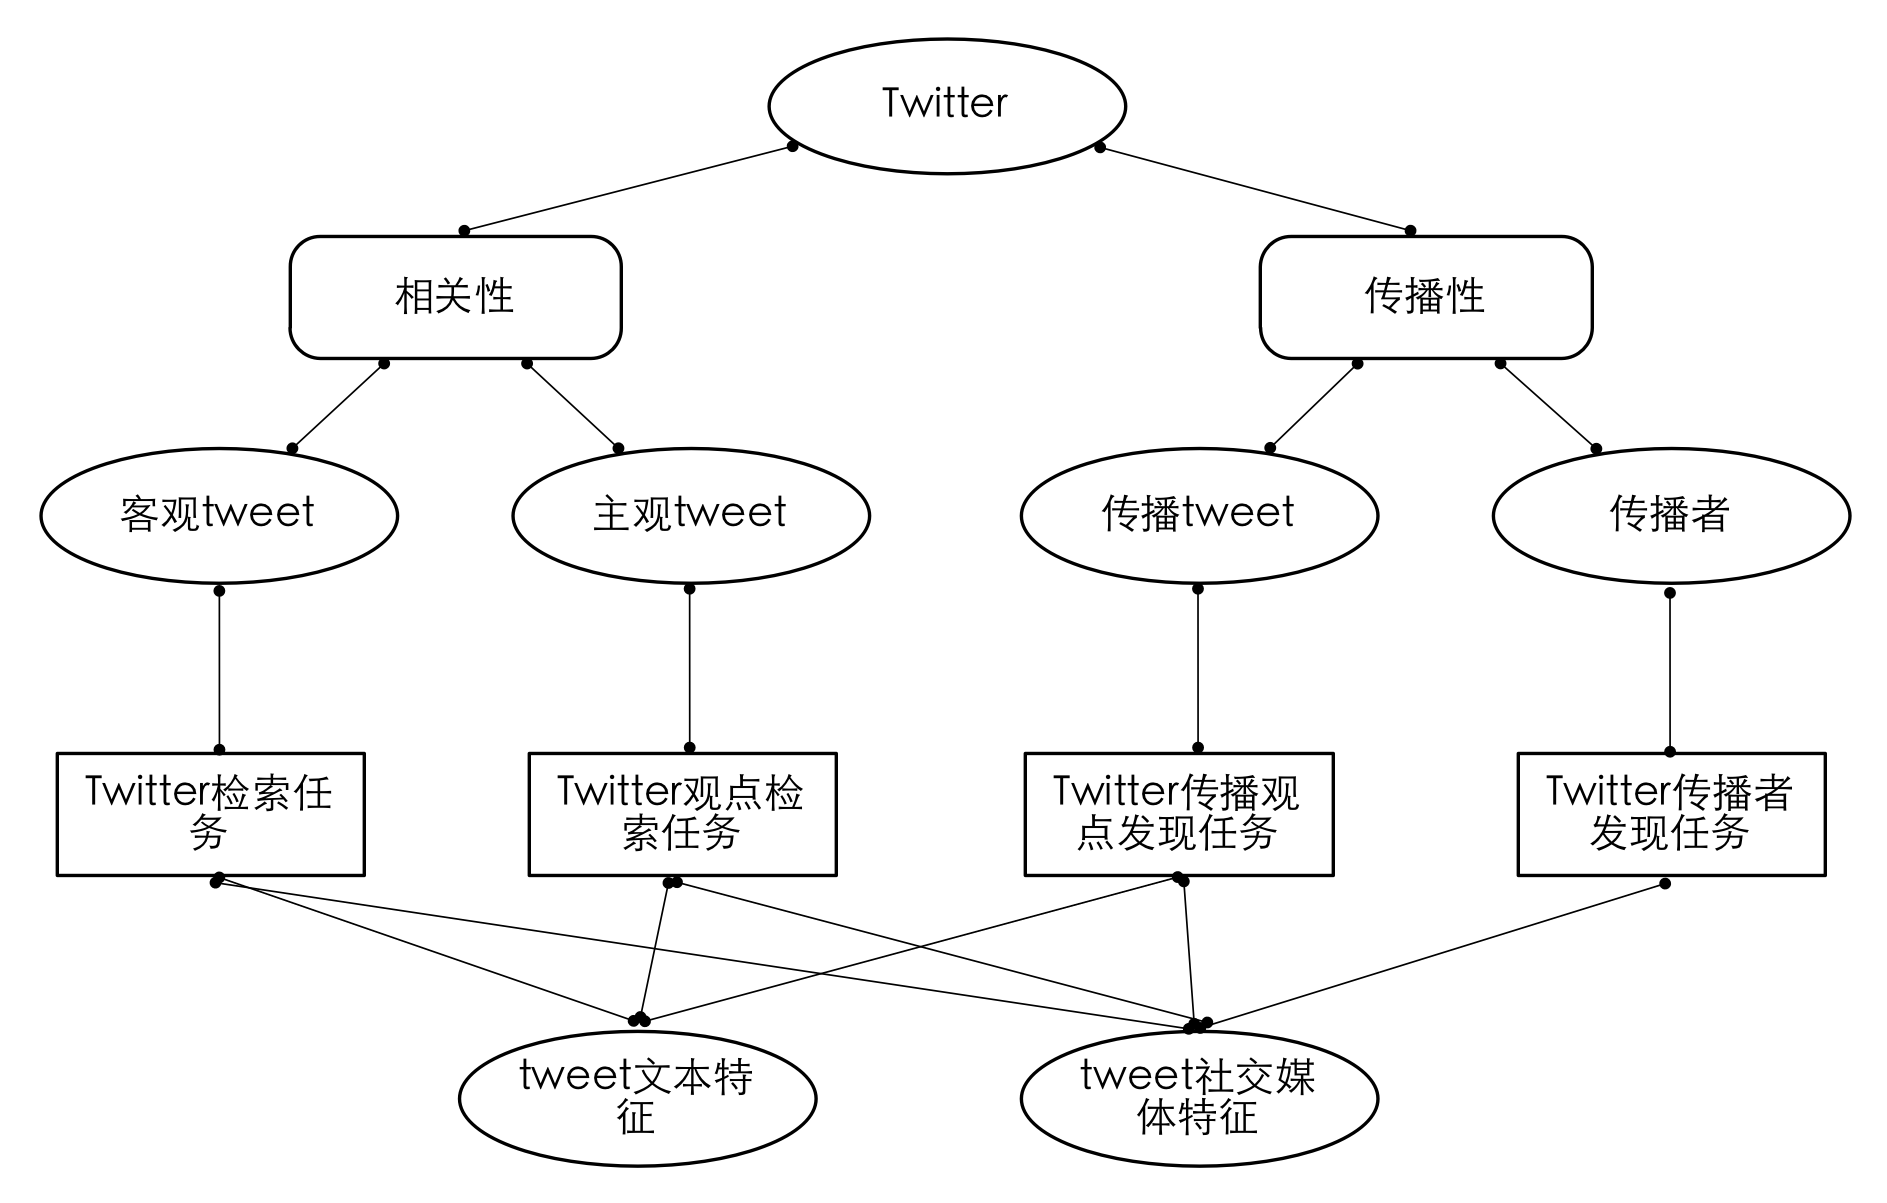
\includegraphics[height=250pt]{Research_Framwork.png}
\caption{本文研究框架}
\label{Research_Framwork}
\end{figure}

具体四个研究内容的定义如下:

\begin{enumerate}
\item \textbf{Twitter检索}:给定关键词,在Twitter中找到话题相关的tweet。通过文本的结构化信息(我们发现tweet文本呈现结构化特点)和社交媒体信息帮助提高Twitter检索,以此分析了人们在Twitter中是如何描述话题以及社交媒体特征与相关话题tweet的内在联系。
\item \textbf{Twitter观点检索}:给定关键词,在Twitter中找到话题相关且带观点的tweet。通过tweet观点化信息(基于结构化信息)和社交媒体信息帮助提高Twitter观点检索,以此分析了人们在Twitter中是如何表达观点以及社交媒体特征与Twitter中观点的内在联系。
\item \textbf{Twitter传播观点发现}:给定关键词,在Twitter中找到话题相关且带观点的tweet,并且这个tweet在未来会被转发。通过tweet观点化信息(基于结构化信息)和社交媒体信息帮助发现Twitter中传播观点,以此分析了人们在Twitter中是如何表达高质量的观点以及社交媒体特征与Twitter中传播观点的内在联系。
\item \textbf{Twitter传播观者发现}:给定tweet,发现tweet的粉丝中,谁会在未来传播这个tweet。通过社交媒体信息帮助发现Twitter中的信息传播者,以此分析了社交媒体特征与Twitter信息传播者的内在联系。
\end{enumerate}

总的来说,针对~\ref{point}的第一个问题,本文通过分析tweet文本的结构化信息和观点表达方式,找出规律与特点,将其利用到Twitter检索、观点检索、传播观点发现任务。
针对~\ref{point}的第二个问题,本文通过分析社交媒体的用户属性、社会网络结构、文本属性,发现用户之间、用户与tweet文本(主客观信息)、用户与传播行为、tweet文本与传播行为之间的内在联系,通过开发社交媒体特征,帮助解决Twitter检索、观点检索、传播观点发现和信息传播者发现任务。

\subsection{本文研究方法}
针对以上研究内容,本文基于自然语言处理技术和机器学习技术,深入分析Twitter中tweet的文本特点和社交媒体属性,解决Twitter中若干检索与传播分析问题。我们希望通过对Twitter中若干检索与传播分析问题的研究达到如下几个主要目标:
\begin{enumerate}
\item 认识以Twitter为代表的社交媒体的新特点,包括文本表现形式,用户属性,Twitter中信息的传播行为等等。
\item 传统的信息检索技术如何在新型的社交媒体中使用,重点研究基于机器学习的信息检索技术在Twitter中的应用。
\item 深入研究Twitter中观点检索问题,寻找人们在Twitter中表达观点的方式,以及其它相关因素。
\item 针对Twitter中tweet文本质量较低,以及质量评价问题,帮助人们进一步理解Twitter中高质量文本的评价问题。
\item 通过研究特定用户查询问题,找到Twitter中tweet、作者和粉丝之间的关系,帮助Twitter中传播分析的研究。
\end{enumerate}  

根据各个具体的研究内容,我们的具体研究方法为:

\begin{enumerate}
\item 针对Twitter中的信息检索问题,我们深入分析tweet中的文本特点,找到文本特定结构与社会属性之间的关系,开发文本结构特征,然后结合tweet的社交媒体特征(用户属性等),将其整合到机器学习的框架中,通过排序学习,提高Twitter中信息检索的效果。
\item 针对Twitter中的观点检索问题,首先对Twitter中的观点检索问题进行定义,构造测试数据集,然后分析Twitter中用户表达观点的文本特点以及Twitter中观点所对应的潜在用户属性,开发特征,利用排序学习,解决Twitter中如何找到观点的问题。
\item 针对Twitter观点检索中大量返回低质量观点的问题,从发现传播观点的角度提出了Twitter中高质量观点的客观评价指标,这个指标利用Twitter中高质量信息大量传播的特点,分析了Twitter传播观点发现的问题,利用tweet中如何判定是否转发的方法,tweet中文本是否包含观点以及tweet文本本身的语言质量帮助相关任务的解决。
\item  针对Twitter中信息传播者发现的问题,我们首先进行问题定义,构造数据集,分析信息传播者的特点,找到信息传播者与转发tweet、转发tweet作者之间的联系,设计相关特征,将其利用到机器学习框架中,解决信息传播者发现的问题。
\end{enumerate}  

\section{本文主要贡献}
本文主要围绕分析Twitter文本的特点与Twitter社交媒体属性展开,通过Twitter中的信息检索和传播分析任务,发现哪些因素能够帮助或影响检索效果的提高与传播分析的准确性。

在tweet文本分析方面,我们发现,虽然tweet是短文本,但是它具有结构化的特点。不同的tweet文本结构对应不同的属性和文本质量,通过挖掘tweet的文本结构信息能够帮助Twitter的信息检索。另外由于某些特定结构的tweet具有某种属性(如主观化),因此可以利用结构化的tweet收集大量的相关文本,构造情感词典帮助tweet主观化判定,提高观点检索的效果。

在Twitter社交媒体属性的分析方面,我们通过对tweet中是否包含链接、hashtag、提及等的研究,确定这些符号串或功能与Twitter信息检索的对应关系,因此帮助该任务的解决。我们还分析了tweet作者的属性,包括作者的粉丝数目、朋友数目、分组数目、兴趣爱好、圈子、活跃时间等等,试图发现这些因素与Twitter信息传播之间的内在联系。

在具体的Twitter信息检索任务中,我们从给定关键词找到主客观相关tweet的两个方面进行研究。获取客观tweet方面,我们开发了tweet文本的结构化特征和社交媒体特征,将其整合到基于排序学习的模型中,实验结果验证了我们的方法是有效的。获取主观tweet即Twitter中的观点检索是一个全新的工作,我们定义了这个问题,发布了关于研究这个问题的实验数据\footnote{下载地址:\url{http://sourceforge.net/p/ortwitter/wiki/Home/}},截止到2013年9月这个实验数据已经有40多个国家和地区超过200多个研究单位和个人下载,并且这个数据还被ICWSM会议推荐为官方的社交媒体研究数据\footnote{\url{http://www.icwsm.org/2013/datasets/datasets/}},针对Twitter中的观点检索我们也提出了我们的方法,主要是开发tweet的文本特征与社交媒体特征结合排序学习框架进行解决,同时我们也提出了一种基于无监督学习的tweet观点化评价的方法,目前有许多其它研究单位的工作围绕我们的Twitter观点检索工作展开\upcite{stajner2013automatic,kothari2013detecting,li2013exploiting,zhang2013personalized}。

在具体的Twitter传播分析任务中,我们从传播的内容和受众两个方面进行考虑,提出了Twitter中传播观点发现的新任务和信息传播者发现的新任务。Twitter中传播观点发现可以帮助我们解决tweet质量评价主观化的问题,由于以往的研究主要是围绕给定tweet,预测该tweet在未来是否会被转发,我们对这个问题进行了细粒度的研究,从观点化的tweet能否被转发的角度进行了探讨,通过开发tweet的文本特征和社交媒体特征解决传播观点发现的问题。Twitter信息传播者发现的问题,针对的是以往研究忽视“谁”会转发的问题,我们定义了这个问题,提出了解决这个问题的方法,发现兴趣与转发的历史信息是决定信息传播者的重要因素,同样我们也公布了研究这个问题的数据集\footnote{下载地址:\url{https://sourceforge.net/projects/retweeter/}},供以后科研人员继续使用。

以上所有的工作都通过论文的形式公开发表\upcite{luo2012improving,luo2012opinion,l2013Luo_POR,Luo:2013:RMF:2484028.2484158}。


\section{本文结构}
本文的研究工作主要围绕社交媒体中检索与传播分析任务展开,我们可以将这两方面的工作分为以下几个主要部分:在Twitter检索方面,我们首先分析了tweet的文本信息与社交媒体信息,以此帮助Twitter中传统的信息检索任务;然后以此为基础,进一步探讨Twitter中观点检索问题,给定关键词,检索到话题相关且带观点的tweet;在Twitter的观点检索任务中,我们发现检索结果存在大量的低质量观点,结合Twitter中的传播分析,我们从传播的内容角度考虑,转发的tweet一般是高质量的信息,因此我们再进一步研究了在Twitter中如何发现传播观点的问题;Twitter信息的传播分析不仅可以从tweet的本身进行研究,也可以从受众的角度进行分析,因此最后我们讨论了在Twiter中如何需找信息传播者的问题。上述工作共分为六个章节,论文主体结构以及章节之间的关系如图~\ref{Paper_Framwork}所示。,每个章节内容具体安排如下:

\begin{figure}[htp]
\centering
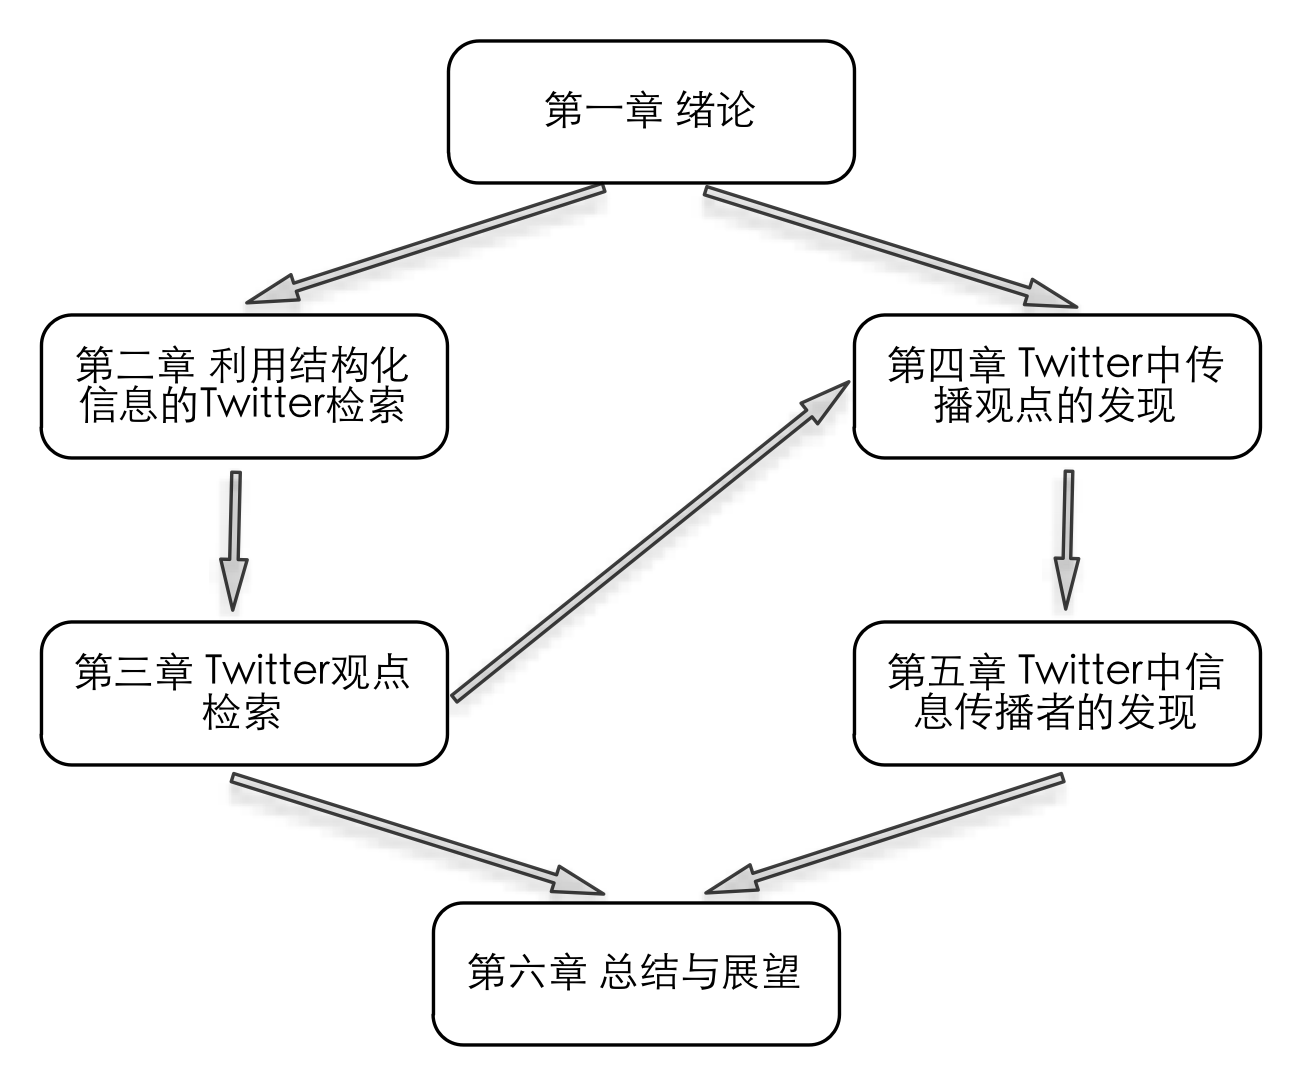
\includegraphics[height=250pt]{Paper_Framwork.png}
\caption{论文整体结构图}
\label{Paper_Framwork}
\end{figure}

第一章是绪论,首先介绍了本文研究的背景,介绍了社交媒体和Twitter的一些基础知识,接着提出研究动机,阐明了本文所涉及的科学问题、研究内容,并给出了研究方法,然后分析了研究问题,确立了依托自然语言处理技术与机器学习方法解决这些问题的基本思路,最后介绍了本文的主要工作和文章的结构。

第二章是Twitter中的信息检索,首先介绍了Twitter信息检索的研究背景,然后提出了以往Twitter信息检索方法忽视tweet文本结构化特点以及存在大量社交媒体信息的问题,以此设计了一种标注tweet文本结构的自动标注器,最后利用自动标注器标注tweet文本开发结构特征,结合社交媒体特征帮助Twitter信息检索,实验验证了方法的有效性。这一章回答了Twitter中
人们是如何用自然语言描述客观话题,并且社交媒体特征与tweet话题相关性存在怎样的联系。

第三章是Twitter中的观点检索,本章开头定义了Twitter中的观点检索问题,分析了Twitter观点检索与以往观点检索的不同特点,接着提出了一种自动获取主观tweet与客观tweet的方法自动生成情感词典,依靠词典对tweet的文本进行主观化判定,结合tweet的用户属性信息和文本信息,利用排序学习算法,实现观点检索。实验部分,我们构造了自己的Twitter观点检索语料,并发布了语料供以后的研究者使用,实验结果证明了我们的观点检索方法有效。这一章回答了Twitter中人们是如何用自然语言表达主观观点,并且社交媒体特征与tweet观点相关性存在怎样的联系。

第四章中我们针对Twitter观点检索存在大量低质量观点的问题,依据转发tweet一般是高质量文本的既有研究成果,提出了在Twitter中发现传播观点的问题。我们首先定义了问题,然后构造了数据集,接着开发了tweet传播度特征、观点化特征和文本质量特征,将其整合到排序学习的机器学习模型框架中。实验结果说明了这些特征对于Twitter中发现传播观点是有帮助的,另外我们的方法可以达到人判定传播观点的效果。这一章回答了Twitter中人们是如何用自然语言表达传播性的观点,并且社交媒体特征与传播性的观点存在怎样的联系。

第五章中我们探讨了Twitter中发现信息传播者的问题,给定一个tweet,发现tweet的作者粉丝中谁会转发该消息。我们开发了转发历史特征 、用户特征、用户活跃时间特征和用户兴趣特征,并依然将其应用到排序学习的框架中构造模型进行排序。实验部分,我们构造了自己的测试数据与基准系统,我们公布了数据,实验结果显示了我们的方法能够成功找到tweet转发者。这一章回答了社交媒体特征与信息传播者存在怎样的联系。

最后一章是总结部分,我们阐明了本文工作的贡献点,并且指出了工作的一些不足,并对未来社交媒体检索与传播分析的一些问题和方法进行了尝试性地思考。


